\section{Phân tích và thiết kế hệ thống}
\subsection{Đề xuất thiết kế hệ thống}
Với mục tiêu đặt ra cũng như những yêu cầu của đồ án thì hệ thống cần có một ứng dụng chạy trên nền tảng Android để làm khối điều khiển trung tâm của Robot với khả năng lấy dữ liệu camera, micro, của thiết bị từ đó tiến hành xử lý với thị giác máy tính để theo dõi, cảnh báo đến người thân khi người được giám sát bị té ngã hay với AI xử lý ngôn ngữ có thể trò chuyện một cách tự nhiên với người được chăm sóc. Ngoài ra ứng dùng này cũng cần có bộ phận xử lý các vấn đề về truyền nhận thông tin hay điều khiển Robot, thiết bị IoT tích hợp mở rộng. 

Hệ thống cũng cần có một ứng dụng (dành cho người thân) để có thể giao tiếp từ xa với Robot, như nhận thông tin về cảnh báo té ngã, lập lịch nhắc nhỡ uống thuốc, gọi video hay thậm chí là điều khiển Robot từ xa để có thể tìm kiếm người thân xung quanh nhà. Mặc dù đây là ứng dụng mà đồ án không yêu cầu và có thể xem xét lược bỏ, tập trung xử lý ở khối điều khiển trung tâm của Robot nhưng với module này hệ thống sẽ hoàn thiện và thực tế hơn.

Với hai module trên thì hệ thống đã tương đối hoàn chỉnh tuy nhiên vẫn cần thêm các hệ thống hạ tầng trung gian để hỗ trợ xử lý chatbot, giọng nói hay cơ sở dữ liệu để lưu trữ thông tin, các giao thức và dịch vụ truyền thông, kết nối như MQTT hay Signaling Server...

\textbf{Hệ thống được chia thành 3 khối chính: Khối Robot (Tại nhà), Hạ tầng Cloud (Trung gian) và Khối điều khiển (Từ xa).}

\textbf{Khối Robot (Tại nhà)}
Đây là thực thể vật lý tương tác trực tiếp với người cao tuổi, bao gồm hai phần chính:
\begin{itemize}
    \item \textbf{Phần cứng Robot:} Đóng vai trò là khung thân vật lý, bao gồm các động cơ, cảm biến, và phần mạch kết nối điều khiển động cơ.
    \item \textbf{Smartphone 1 (Bộ não Robot):} Sử dụng một điện thoại Android làm trung tâm xử lý chính. Trên này chạy Ứng dụng Android Robot tích hợp các công nghệ AI quan trọng:
    \begin{itemize}
        \item \textit{AI Thị giác máy tính:} Thực hiện các tác vụ xử lý tại biên (Edge Computing) như phát hiện té ngã và theo dõi người dùng (tracking).
        \item \textit{AI Xử lý ngôn ngữ:} Nhận dạng giọng nói và vận hành Chatbot để giao tiếp với người già.
        \item \textit{Hệ thống truyền tin, điều khiển:} Là cầu nối trung gian để gửi lệnh điều khiển xuống phần cứng Robot, truyền thông tin liên quan camera, micro đến các khối liên quan.
    \end{itemize}
\end{itemize}

\textbf{Hạ tầng Cloud (Trung gian)}
Đóng vai trò là "trạm trung chuyển" dữ liệu và cung cấp khả năng lưu trữ, hỗ trợ xử lý các tác vụ liên quan đến chatbot:
\begin{itemize}
    \item \textbf{MQTT Broker:} Giao thức thông tin nhẹ, chuyên dùng để truyền các lệnh điều khiển từ người nhà đến robot hoặc gửi các cảnh báo khẩn cấp đến người nhà.
    \item \textbf{Signaling Server:} Phục vụ cho việc thiết lập kết nối truyền tải hình ảnh/video (Video Streaming) giữa Robot ứng dụng Caregiver
    \item \textbf{Cơ sở dữ liệu (Database):} Lưu trữ các thông tin quan trọng như lịch uống thuốc, nhật ký hoạt động (logs) và dữ liệu người dùng.
    \item \textbf{Cloud NLP Service:} Hỗ trợ xử lý ngôn ngữ tự nhiên nâng cao cho Chatbot.
\end{itemize}

\textbf{Khối Điều khiển Robot (Từ xa)}
Đây là giao diện dành cho người chăm sóc (Caregiver) để theo dõi và hỗ trợ người cao tuổi từ xa thông qua \textbf{Smartphone 2} chạy ứng dụng Android Caregiver:
\begin{itemize}
    \item \textbf{Bảng điều khiển (Virtual Joystick):} Điều khiển Robot di chuyển thủ công trong nhà.
    \item \textbf{Màn hình Video call:} Quan sát không gian xung quanh để có thể điều khiển Robot di chuyển và trò chuyện với người cao tuổi.
    \item \textbf{Nhận cảnh báo:} Nhận thông báo ngay lập tức nếu robot phát hiện người thân bị té ngã hoặc có bất thường.
    \item \textbf{Lập lịch nhắc nhở:} Cài đặt lịch uống thuốc hoặc các mốc thời gian quan trọng để robot nhắc nhở người cao tuổi tại nhà.
    
\end{itemize}
\begin{figure}[htbp]
    \centering
    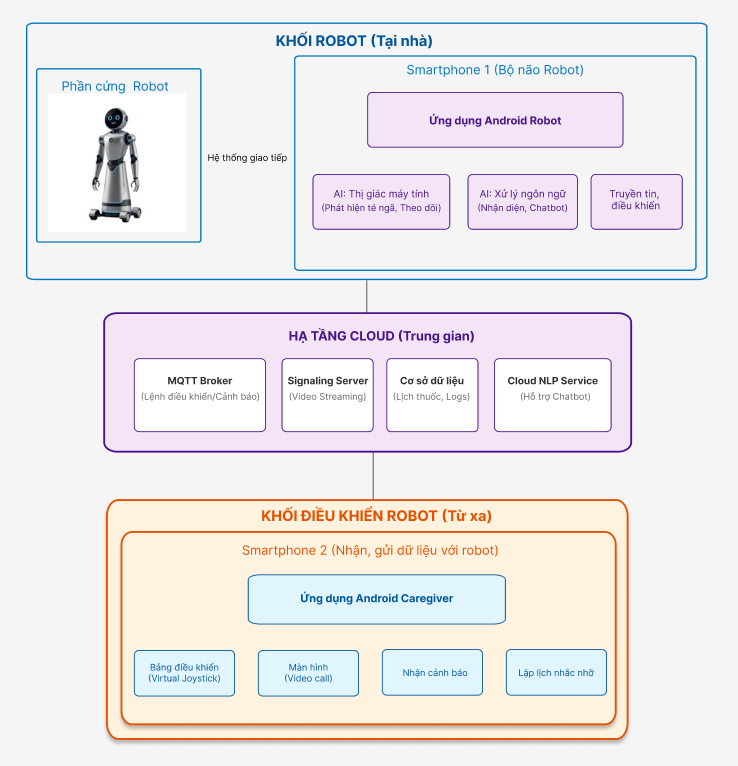
\includegraphics[width=1\textwidth]{Images/sơ đồ hệ thống.png}
    \caption{Thiết kế hệ thống đề xuất}
\end{figure}
\newpage
\subsection{Đề xuất giải pháp cho chức năng phát hiện té ngã}
\subsubsection{Lựa chọn YOLOv11 cho chức năng phát hiện té ngã}

\textbf{a) Thuộc nhóm State-of-the-Art (SOTA)}

YOLOv11 đạt hiệu suất SOTA trên các benchmark chuẩn như COCO 2017 [11]. So với các phiên bản trước:
\begin{itemize}
    \item Độ chính xác cao hơn YOLOv8 khoảng 1-2\% mAP với cùng kích thước mô hình
    \item Số lượng parameters giảm 22\% so với YOLOv8 (YOLOv11m: 20.1M vs YOLOv8m: 25.9M)
    \item Tốc độ inference nhanh hơn 10-15\% nhờ tối ưu hóa module C3k2
\end{itemize}

\textbf{Bảng so sánh benchmark với các thế hệ YOLO:}

\begin{table}[h!]
\centering
\begin{tabular}{|l|c|c|c|c|}
\hline
\textbf{Model} & \textbf{Params (M)} & \textbf{mAP$_{50-95}$} & \textbf{Latency (ms)} & \textbf{Năm} \\
\hline
YOLOv5m & 21.2 & 45.4\% & 4.0 & 2020 \\
\hline
YOLOv7-M & 36.9 & 51.4\% & 6.1 & 2022 \\
\hline
YOLOv8m & 25.9 & 50.2\% & 4.2 & 2023 \\
\hline
YOLOv9m & 20.0 & 51.4\% & 4.5 & 2024 \\
\hline
YOLOv10m & 16.5 & 51.3\% & 3.5 & 2024 \\
\hline
\rowcolor{yellow!20}
\textbf{YOLOv11m} & \textbf{20.1} & \textbf{51.5\%} & \textbf{4.7} & \textbf{2024} \\
\hline
\end{tabular}
\label{tab:yolo_benchmark_comparison}
\end{table}

Từ bảng benchmark, YOLOv11 cho thấy:
\begin{itemize}
    \item Đạt mAP cao nhất (51.5\%) trong các phiên bản YOLO
    \item Hiệu quả parameters tốt hơn YOLOv8 (ít hơn 22\% params nhưng mAP cao hơn)
    \item Cân bằng tốt giữa accuracy và speed
\end{itemize}


\textbf{b) Cải tiến về Non-Maximum Suppression (NMS)}

Các phiên bản YOLO truyền thống sử dụng NMS như bước hậu xử lý để loại bỏ các bounding box trùng lặp. NMS có nhược điểm:
\begin{itemize}
    \item Là thao tác tuần tự, không song song hóa được trên GPU
    \item Tạo bottleneck trong quá trình inference
    \item Cần tinh chỉnh ngưỡng IoU, ảnh hưởng đến kết quả
\end{itemize}

YOLOv11 tích hợp các cơ chế giảm phụ thuộc vào NMS thông qua loss function và kiến trúc head được thiết kế để giảm thiểu các prediction trùng lặp ngay từ đầu.

\textbf{c) Tốc độ suy luận nhanh, phù hợp thời gian thực}

Trong ứng dụng phát hiện ngã, thời gian phản hồi là yếu tố sống còn. YOLOv11 đạt:
\begin{itemize}
    \item Hàng trăm FPS trên GPU hiện đại (RTX 3060 trở lên)
    \item Có thể chạy trên thiết bị edge như Jetson Nano với tốc độ chấp nhận được
    \item Latency thấp, phù hợp cho hệ thống giám sát cần cảnh báo tức thì
\end{itemize}

\textbf{d) Hiệu quả trên video giám sát}

Video giám sát trong nhà thường có đặc điểm:
\begin{itemize}
    \item Góc camera cố định, background ít thay đổi
    \item Ánh sáng không đều, có thể thiếu sáng
    \item Đối tượng (người) chiếm phần lớn khung hình
\end{itemize}

YOLOv11 được huấn luyện với data augmentation mạnh mẽ (mosaic, mixup, photometric distortion), giúp mô hình robust với các điều kiện này.


\subsubsection{Lựa chọn YOLOv11n cho Robot}

Đồ án này lựa chọn \textbf{YOLOv11n} (nano) thay vì các phiên bản lớn hơn vì các lý do sau:

\begin{itemize}
    \item \textbf{Phù hợp với nền tảng Robot}: Robot sử dụng smartphone làm bộ xử lý chính, YOLOv11n với chỉ 2.6M parameters có thể chạy mượt mà trên điện thoại Android
    
    \item \textbf{Real-time trên thiết bị nhúng}: Đạt 25-45 FPS trên smartphone với TensorFlow Lite, đủ cho giám sát thời gian thực
    
    \item \textbf{Tiết kiệm pin}: Model nhẹ tiêu thụ ít năng lượng hơn, quan trọng cho robot di động sử dụng pin
    
    \item \textbf{Độ chính xác chấp nhận được}: mAP 39.5\% đủ tốt cho bài toán Fall Detection (chỉ cần phân biệt fall/no\_fall)
    
    \item \textbf{Latency thấp}: 1.55ms cho phép phản hồi nhanh trong trường hợp khẩn cấp
    
    \item \textbf{Dễ fine-tune}: Model nhỏ huấn luyện nhanh hơn trên GPU tầm trung, ít overfitting hơn trên dataset nhỏ như CauCaFall
\end{itemize}

\textbf{Ước tính FPS của YOLOv11n trên các nền tảng:}

\begin{center}
\begin{tabular}{|l|c|c|}
\hline
\textbf{Nền tảng} & \textbf{FPS ước tính} & \textbf{Ghi chú} \\
\hline
GPU NVIDIA (TensorRT) & 400-600 & RTX 3060+ \\
GPU NVIDIA (PyTorch) & 150-250 & RTX 2060+ \\
Apple CoreML & 40-100 & iPhone 12+ \\
Android (TFLite) & 25-45 & Snapdragon 8xx \\
CPU (ONNX) & 15-20 & Intel i7 \\
Jetson Nano & 10-15 & Edge deployment \\
\hline
\end{tabular}
\end{center}

\textit{Ghi chú: FPS thực tế phụ thuộc vào kích thước ảnh đầu vào (mặc định 640x640) và điều kiện phần cứng.}

\subsection{Đề xuất giải pháp cho chức năng theo dõi(tracking)}
\subsubsection{Các thuật toán Tracking phổ biến}

Trong lĩnh vực Multi-Object Tracking (MOT), có nhiều thuật toán đã được phát triển. Bảng sau so sánh các thuật toán tracking phổ biến:

\begin{table}[h!]
\centering
\caption{So sánh các thuật toán Multi-Object Tracking}
\small
\begin{tabular}{|l|c|c|c|c|c|c|}
\hline
\textbf{Thuật toán} & \textbf{Motion} & \textbf{Appearance} & \textbf{MOTA} & \textbf{FPS} & \textbf{ReID} & \textbf{Năm} \\
\hline
SORT & Kalman Filter & Không & 74.6 & 260 & Không & 2016 \\
\hline
DeepSORT & Kalman Filter & Deep CNN & 75.4 & 20 & Có & 2017 \\
\hline
\textbf{ByteTrack} & \textbf{Kalman Filter} & \textbf{Không} & \textbf{80.3} & \textbf{30} & \textbf{Không} & \textbf{2022} \\
\hline
OC-SORT & Kalman + ORU & Không & 78.0 & 28 & Không & 2022 \\
\hline
BoT-SORT & Kalman + CMC & BoT features & 80.5 & 15 & Có & 2022 \\
\hline
\end{tabular}
\label{tab:tracking_comparison}
\end{table}

\textit{Benchmark trên MOT17 test set}

Đồ án này lựa chọn \textbf{ByteTrack} [5] làm thuật toán tracking chính vì đạt cân bằng tốt nhất giữa độ chính xác và tốc độ, đồng thời không yêu cầu mạng Re-identification phụ.

\subsubsection{Chi tiết thuật toán ByteTrack}

ByteTrack [5] được đề xuất bởi Zhang et al. (ECCV 2022) với ý tưởng đột phá: \textit{tận dụng cả các detection có confidence thấp} thay vì loại bỏ chúng như các tracker truyền thống.

\textbf{Vấn đề với các tracker truyền thống:}
\begin{itemize}
    \item Các tracker như SORT, DeepSORT chỉ sử dụng detection có confidence cao (thường $> 0.5$)
    \item Detection thấp bị loại bỏ, gây mất track khi đối tượng bị che khuất một phần
    \item Dẫn đến ID switch và fragmentation cao
\end{itemize}

\textbf{Ý tưởng cốt lõi của ByteTrack:}

\begin{quote}
``Every detection box, including the low score ones, is a true positive if they match correctly.''
\end{quote}

\textbf{Thuật toán BYTE (2-stage association):}

ByteTrack thực hiện association hai giai đoạn:

\begin{enumerate}
    \item \textbf{Giai đoạn 1 - High score matching}:
    \begin{itemize}
        \item Lọc các detection có score $\geq \tau_{high}$ (thường $\tau_{high} = 0.6$)
        \item Dùng Kalman Filter dự đoán vị trí các track hiện có
        \item Ghép nối high-score detections với tracks bằng Hungarian Algorithm + IoU
        \item Các track không match được chuyển sang giai đoạn 2
    \end{itemize}
    
    \item \textbf{Giai đoạn 2 - Low score matching}:
    \begin{itemize}
        \item Lọc các detection có score trong khoảng $[\tau_{low}, \tau_{high})$ (thường $\tau_{low} = 0.1$)
        \item Ghép nối low-score detections với \textit{unmatched tracks} từ giai đoạn 1
        \item Điều này giúp duy trì track khi đối tượng bị occluded (detection score thấp)
    \end{itemize}
\end{enumerate}

\textbf{Pseudo-code ByteTrack:}
\begin{verbatim}
Input: Detections D, Tracks T, thresholds τ_high, τ_low
Output: Updated Tracks T'

1. D_high = {d in D | d.score >= τ_high}
2. D_low  = {d in D | τ_low <= d.score < τ_high}

# Stage 1: Match high-score detections
3. Predict track positions using Kalman Filter
4. Compute IoU cost matrix between D_high and T
5. Match using Hungarian Algorithm
6. T_matched, T_unmatched, D_unmatched = Assignment

# Stage 2: Match low-score detections  
7. Compute IoU cost matrix between D_low and T_unmatched
8. Match using Hungarian Algorithm
9. Update T_matched with matched low-score detections

# Post-processing
10. Initialize new tracks from D_unmatched (high-score)
11. Mark T_unmatched as lost (delete if lost > max_age)

\end{verbatim}

\textbf{Lý do chọn ByteTrack cho hệ thống Fall Detection:}
\begin{enumerate}
    \item \textbf{Cân bằng tốc độ-chính xác}: MOTA 80.3\% với 30 FPS, đủ cho real-time trên smartphone
    \item \textbf{Không cần ReID network}: Giảm độ phức tạp và tài nguyên tính toán
    \item \textbf{Xử lý occlusion tốt}: Low-score matching giúp duy trì track khi người ngã (confidence thường giảm do tư thế bất thường)
    \item \textbf{Dễ tích hợp}: Chỉ cần YOLOv11 detection + ByteTrack, không cần model phụ
    \item \textbf{ID switch thấp}: Chỉ 159 ID switches trên MOT17, quan trọng cho việc theo dõi liên tục người cao tuổi
\end{enumerate}

\subsubsection{Person Re-identification (ReID)}

Person Re-identification (ReID) là bài toán nhận diện lại cùng một người từ các camera khác nhau hoặc sau khi người đó ra khỏi và quay lại khung hình. Đây là thành phần quan trọng để duy trì identity người dùng trong hệ thống giám sát đa camera.

\textbf{Kiến trúc hệ thống ReID:}

\begin{enumerate}
    \item \textbf{Feature Extraction (Trích xuất đặc trưng)}:
    \begin{itemize}
        \item Backbone CNN (ResNet-50, OSNet) trích xuất visual features từ ảnh người
        \item Output: Embedding vector 256-2048 chiều đại diện cho appearance
        \item Có thể bổ sung local features từ các phần cơ thể (head, torso, legs)
    \end{itemize}
    
    \item \textbf{Metric Learning (Học khoảng cách)}:
    \begin{itemize}
        \item \textbf{Triplet Loss}: Kéo gần các ảnh cùng người, đẩy xa các ảnh khác người
        \begin{equation}
        L_{triplet} = \max(0, d(a, p) - d(a, n) + \alpha)
        \end{equation}
        với $a$: anchor, $p$: positive, $n$: negative, $\alpha$: margin
        \item \textbf{Contrastive Loss}: So sánh từng cặp ảnh positive/negative
        \item \textbf{Center Loss}: Giảm intra-class variation
    \end{itemize}
    
    \item \textbf{Gallery Matching (So khớp)}:
    \begin{itemize}
        \item Query image được so sánh với gallery database chứa các ID đã biết
        \item Cosine similarity hoặc Euclidean distance để ranking
        \item Re-ranking techniques để cải thiện kết quả
    \end{itemize}
\end{enumerate}

\textbf{Bảng so sánh các mô hình ReID phổ biến:}

\begin{table}[h!]
\centering
\caption{So sánh các mô hình Person Re-identification}
\small
\begin{tabular}{|l|c|c|c|c|}
\hline
\textbf{Mô hình} & \textbf{Backbone} & \textbf{mAP} & \textbf{FPS} & \textbf{Đặc điểm} \\
\hline
OSNet & Custom lightweight & 84.9\% & 100+ & Nhẹ, phù hợp real-time \\
\hline
AGW & ResNet-50 + Attention & 87.8\% & 50 & Global-local features \\
\hline
TransReID & ViT + Side info & 89.5\% & 30 & SOTA accuracy \\
\hline
FastReID & ResNet-50 & 86.4\% & 80 & Easy deployment \\
\hline
\end{tabular}
\label{tab:reid_comparison}
\end{table}

\textit{Benchmark trên Market-1501 dataset}


\subsection{Đề xuất giải pháp cho chức năng xử lý ngôn ngữ, giao tiếp}

\textbf{Quy trình xử lý ngôn ngữ tự nhiên (NLP Pipeline)}
Để robot có khả năng nghe - hiểu và phản hồi tự nhiên, hệ thống triển khai quy trình ba bước:
\begin{itemize}
    \item \textbf{Nhận dạng giọng nói (ASR - Automatic Speech Recognition):} Sử dụng \textit{Google Speech-to-Text API} tích hợp trực tiếp trên Smartphone 1. Công nghệ này hỗ trợ tốt tiếng Việt đa vùng miền và có khả năng xử lý tốt trong môi trường có tiếng ồn nền.
    \item \textbf{Xử lý hội thoại (Cloud NLP Service):} Sau khi chuyển âm thanh thành văn bản, dữ liệu được gửi lên Cloud để xử lý thông qua API của các mô hình ngôn ngữ lớn (LLM) như \textit{OpenAI} hoặc \textit{Google Cloud}. Lựa chọn này giúp robot có khả năng hiểu ngữ cảnh sâu, đưa ra lời khuyên về sức khỏe hoặc trò chuyện tâm sự với người già thay vì chỉ phản hồi theo kịch bản cứng nhắc.
    \item \textbf{Tổng hợp giọng nói (TTS - Text-to-Speech):} Sử dụng \textit{Google TTS} hoặc \textit{FPT.AI} để chuyển văn bản phản hồi thành giọng nói. Ưu tiên sử dụng các giọng đọc vùng miền (Bắc/Trung/Nam) tự nhiên để tạo cảm giác gần gũi cho người dùng.
\end{itemize}

% \subsubsection{Tích hợp AI Agent với Robot}

% Kiến trúc tích hợp AI Agent vào hệ thống Robot bao gồm ba khối chính như minh họa trong sơ đồ hệ thống:

% \begin{enumerate}
%     \item \textbf{Khối Robot (Tại nhà)}:
%     \begin{itemize}
%         \item Phần cứng robot kết nối với Smartphone 1 (Bộ não Robot)
%         \item AI Thị giác máy tính: Phát hiện té ngã, theo dõi người (YOLOv11 + ByteTrack)
%         \item AI Xử lý ngôn ngữ: Nhận dạng giọng nói, Chatbot (STT + LLM)
%         \item Module truyền tin và điều khiển IoT
%     \end{itemize}
    
%     \item \textbf{Hạ tầng Cloud (Trung gian)}:
%     \begin{itemize}
%         \item MQTT Broker: Trung chuyển lệnh điều khiển và cảnh báo
%         \item Signaling Server: Hỗ trợ video streaming (WebRTC)
%         \item Cơ sở dữ liệu: Lưu trữ lịch thuốc, logs hoạt động
%         \item Cloud NLP Service: API LLM cho chatbot thông minh
%     \end{itemize}
    
%     \item \textbf{Khối Điều khiển Robot (Từ xa)}:
%     \begin{itemize}
%         \item Smartphone 2 với ứng dụng Android Caregiver
%         \item Bảng điều khiển (Virtual Joystick), Video call, Nhận cảnh báo, Lập lịch nhắc nhở
%     \end{itemize}
% \end{enumerate}

% \textbf{Luồng xử lý AI Agent (System Flow):}

% \begin{enumerate}
%     \item \textbf{Input Processing}:
%     \begin{itemize}
%         \item Speech-to-Text (Whisper/Google STT) chuyển giọng nói thành văn bản
%         \item Computer Vision (YOLOv11) phân tích hình ảnh và video real-time
%     \end{itemize}
    
%     \item \textbf{AI Agent Core - LLM Processing}:
%     \begin{itemize}
%         \item LLM API (GPT-4o, Gemini) xử lý ngôn ngữ tự nhiên
%         \item RAG truy xuất thông tin cá nhân hóa (lịch thuốc, sở thích)
%         \item Memory module lưu trữ ngữ cảnh hội thoại
%     \end{itemize}
    
%     \item \textbf{NLP Output Processing cho điều khiển IoT}:
%     \begin{itemize}
%         \item Phân tích output text từ LLM API
%         \item Keyword matching để xác định action
%         \item Gửi command tương ứng qua MQTT
%     \end{itemize}
    
%     \item \textbf{Action Execution}:
%     \begin{itemize}
%         \item Text-to-Speech (Edge Speech-to-Text) phản hồi bằng giọng nói
%         \item Robot Control API điều khiển di chuyển
%         \item MQTT publish lệnh đến thiết bị IoT
%     \end{itemize}
% \end{enumerate}

\subsection{Đề xuất các giao thức giao tiếp sử dụng}

Trong quá trình nghiên cứu và phát triển hệ thống, một số giao thức truyền giao tiếp được sử dụng để giải quyết các vấn đề kết nối, giao tiếp giữa các module trong hệ thống.

\subsubsection{Giao thức MQTT (Message Queuing Telemetry Transport)}
Đây là giao thức chủ đạo được sử dụng để truyền tải dữ liệu điều khiển và cảnh báo thông qua MQTT Broker trung gian.
\begin{itemize}
    \item \textbf{Ứng dụng:} Truyền lệnh điều khiển từ giao diện bảng điều khiển (Virtual Joystick) trên thiết bị của người thân đến Robot. Đồng thời, Robot sử dụng giao thức này để gửi các cảnh báo khẩn cấp (như phát hiện té ngã) về ứng dụng giám sát.
    \item \textbf{Ưu điểm:} Tiết kiệm băng thông, tiêu tốn ít năng lượng, hoạt động hiệu quả trong điều kiện mạng không ổn định, đặc biệt phù hợp cho các thiết bị IoT và di động.
\end{itemize}

\subsubsection{Giao thức WebRTC (Real-Time Communication)}
Giao thức này được triển khai thông qua Signaling Server để thiết lập các kênh truyền thông đa phương tiện thời gian thực.
\begin{itemize}
    \item \textbf{Ứng dụng:} Hỗ trợ tính năng truyền hình ảnh trực tiếp (Video Streaming) và đàm thoại video (Video Call), cho phép người thân giám sát trực tiếp qua camera của robot với độ trễ cực thấp.
    \item \textbf{Cơ chế:} Sử dụng Signaling Server để thực hiện quá trình bắt tay (handshake) giữa hai thiết bị Android, sau đó dữ liệu video được truyền trực tiếp theo mô hình ngang hàng (Peer-to-Peer) để tối ưu hóa tốc độ.
\end{itemize}

\subsubsection{Giao thức HTTP/HTTPS}
Được sử dụng làm cầu nối giao tiếp chính với hệ thống cơ sở dữ liệu và các dịch vụ tính toán đám mây.
\begin{itemize}
    \item \textbf{Ứng dụng:} 
    \begin{itemize}
        \item Đồng bộ hóa dữ liệu về lịch nhắc nhở y tế, nhật ký hoạt động (Logs) của người cao tuổi.
        \item Gửi yêu cầu xử lý ngôn ngữ tự nhiên (NLP) lên Cloud để nhận phản hồi thông minh từ hệ thống Chatbot.
    \end{itemize}
    \item \textbf{Ưu điểm:} Khả năng tương thích cao với các dịch vụ đám mây hiện đại, đảm bảo tính toàn vẹn và an toàn dữ liệu thông qua mã hóa SSL/TLS.
\end{itemize}

\subsubsection{Giao tiếp nội bộ (Serial/Bluetooth)}
Tại Robot, việc truyền tín hiệu giữa Smartphone đóng vai trò "bộ não" và phần cứng điều khiển động cơ được thực hiện qua các chuẩn kết nối tầm ngắn.
\begin{itemize}
    \item \textbf{Ứng dụng:} Thực hiện việc giao tiếp giữa Smartphone và phần cứng Robot. 
    \item \textbf{Chuẩn kết nối:} Ưu tiên sử dụng giao tiếp Serial (UART) thông qua cổng kết nối vật lý giúp đảm bảo tin cậy và tốc độ cao hoặc giao thức Bluetooth.
\end{itemize}

% \subsubsection{Kết nối Internet (TCP/IP)}
% Toàn bộ các thành phần trong hệ thống, bao gồm Robot và ứng dụng người thân, luôn duy trì kết nối thông qua môi trường mạng Wi-Fi hoặc 4G/5G. Đây là nền tảng giao thức cơ bản đảm bảo khả năng kết nối xuyên suốt và đồng bộ dữ liệu với hạ tầng Cloud trung tâm.

% Để đảm bảo tín đơn giản dễ hiện thực của đồ án

\subsubsection{Kết nối Internet (TCP/IP)}

Toàn bộ các thành phần trong hệ thống, bao gồm Robot (Smartphone 1) và ứng dụng người thân (Smartphone 2), luôn duy trì kết nối thông qua giao thức TCP/IP trên nền tảng mạng Wi-Fi hoặc 4G/5G. Đây là nền tảng hạ tầng cốt lõi đảm bảo khả năng kết nối xuyên suốt và đồng bộ dữ liệu với các dịch vụ trên Cloud. Một số ưu và nhược điểm của hai phương thức kết nối như sau:

\begin{itemize}
    \item \textbf{Mạng không dây Wi-Fi:}
    \begin{itemize}
        \item \textit{Ưu điểm:} Cung cấp băng thông lớn và ổn định, đặc biệt quan trọng cho việc truyền tải luồng dữ liệu đa phương tiện (Video Call/Streaming) qua WebRTC với độ phân giải cao. Chi phí vận hành thấp và giúp tiết kiệm điện năng cho Smartphone hơn so với mạng di động.
        \item \textit{Nhược điểm:} Phạm vi phủ sóng bị hạn chế trong không gian gia đình, tín hiệu có thể bị suy giảm khi Robot di chuyển qua các vật cản như tường hoặc cửa.
    \end{itemize}
    
    \item \textbf{Mạng di động (4G/5G):}
    \begin{itemize}
        \item \textit{Ưu điểm:} Đảm bảo tính linh động tối đa cho ứng dụng người thân (Caregiver App), cho phép giám sát và nhận cảnh báo té ngã từ Robot ở bất cứ đâu có sóng di động. 5G mang lại ưu thế về độ trễ cực thấp, hỗ trợ tốt cho việc điều khiển Robot qua MQTT thời gian thực.
        \item \textit{Nhược điểm:} Độ trễ (Latency) và độ biến thiên trễ có thể thay đổi tùy thuộc vào khu vực và nhà mạng, ảnh hưởng đến sự đồng bộ của video. Ngoài ra, việc sử dụng liên tục sẽ tiêu tốn nhiều năng lượng và phát sinh chi phí dữ liệu di động.
    \end{itemize}
\end{itemize}

Trong ứng dụng thực tế Robot có thể ưu tiên sử dụng mạng di động để đảm bảo tính tin cậy khi có sự cố mất điện tuy nhiên một số khác lại ưu tiên vấn đề chi chí hay tiêu tốn pin. Còn trong bối cảnh đồ án này nên ưu tiên sử dụng kết nối Wifi để triển khai dễ dàng, tiết kiệm hơn.

\subsection{Vấn đề liên quan mất đồng bộ giữa tín hiệu điều khiển Robot và Video call}

Tín hiệu điều khiển robot qua MQTT và video robot truyền về người điều khiển qua WebRTC có tốc độ khác nhau, gây ra vấn đề mất đồng bộ. Phần này đề xuất các giải pháp đảm bảo hệ thống chạy ổn định.

\textbf{1. Vấn đề mất đồng bộ:}

Thách thức về sự mất đồng bộ nảy sinh khi có sự sai lệch về thời gian truyền dẫn giữa giao thức MQTT (điều khiển) và WebRTC (video). Sự mất cân bằng này tạo ra "độ trễ thị giác", khiến người điều khiển không thể nắm bắt chính xác trạng thái thực tế của Robot trong không gian, từ đó gia tăng rủi ro hư hại thiết bị do va đập. Chính vì thế, việc kiểm soát và đồng bộ hóa các luồng tín hiệu là một nhiệm vụ quan trọng để nâng cao hiệu quả vận hành từ xa.
\begin{itemize}
    \item \textbf{MQTT (TCP)}: Tín hiệu điều khiển đi qua Cloud broker
    \item \textbf{WebRTC (UDP)}: Video streaming P2P
    \item Hai luồng dữ liệu độc lập với tốc độ và đường truyền khác nhau
\end{itemize}

\textbf{2. Giải pháp Timestamp và Cảnh báo Kết nối:}

Mỗi gói tin điều khiển gửi qua MQTT và mỗi khung hình WebRTC đều được gắn nhãn thời gian (timestamp). Khi ứng dụng người thân nhận được, nó sẽ tính toán độ lệch trễ:

\begin{equation}
\Delta t = t_{receive} - t_{send}
\end{equation}

Trong đó:
\begin{itemize}
    \item $t_{send}$: Thời điểm gửi gói tin từ robot
    \item $t_{receive}$: Thời điểm nhận được tại ứng dụng người thân
    \item $\Delta t$: Độ trễ thực tế của kết nối
\end{itemize}

\textbf{Cơ chế cảnh báo:}
\begin{itemize}
    \item Nếu $\Delta t < 100ms$: Kết nối tốt, điều khiển bình thường
    \item Nếu $100ms \leq \Delta t < 300ms$: Kết nối trung bình, hiển thị cảnh báo nhẹ
    \item Nếu $\Delta t \geq 300ms$: Cảnh báo ``\textit{Kết nối yếu}'' để người dùng giảm tốc độ điều khiển
    \item Các ngưỡng thời gian đưa ra cảnh báo có thể thay đổi khi tiến hành chạy thực nghiệm
\end{itemize}

\textbf{3. Giải pháp Cảm biến Phần cứng (Collision Avoidance):}

Để đảm bảo an toàn khi có độ trễ lớn, khối phần cứng Robot được tích hợp cảm biến siêu âm hoặc hồng ngoại để tự động tránh vật cản:

\begin{itemize}
    \item \textbf{Cảm biến siêu âm}: thường đo khoảng cách từ 3cm đến 400cm
    \item \textbf{Cảm biến hồng ngoại}: thường phát hiện vật cản ở khoảng cách gần ($<$30cm)
\end{itemize}

\textbf{Một số ưu nhược điểm của từng cảm biến:}

\begin{itemize} 
\item \textbf{Cảm biến siêu âm (Ultrasonic Sensor):} 
\begin{itemize} \item \textit{Ưu điểm:} Có phạm vi đo đạc rộng (lên đến 400cm), cho phép Robot nhận biết vật cản từ xa để giảm tốc độ dần đều thay vì dừng đột ngột. Đặc biệt, cảm biến không bị ảnh hưởng bởi màu sắc hay độ trong suốt của vật cản (như cửa kính). \item \textit{Nhược điểm:} Tốc độ phản hồi phụ thuộc vào tốc độ âm thanh nên chậm hơn so với cảm biến ánh sáng. Có thể xảy ra hiện tượng "góc chết" khi gặp các bề mặt không phẳng gây tán xạ âm hoặc các bề mặt hấp thụ âm như rèm cửa, thảm trải sàn. 
\end{itemize}  

\item \textbf{Cảm biến hồng ngoại (Infrared Sensor):}
\begin{itemize}
    \item \textit{Ưu điểm:} Kích thước nhỏ gọn, chi phí thấp và tốc độ phản hồi cực nhanh do sử dụng tín hiệu ánh sáng. Đây là giải pháp tối ưu cho việc phát hiện vật cản ở cự ly gần để kích hoạt dừng khẩn cấp.
    \item \textit{Nhược điểm:} Phạm vi hoạt động hẹp ($<$30-80cm). Độ chính xác bị ảnh hưởng nghiêm trọng bởi ánh sáng môi trường (ánh nắng mặt trời) và màu sắc của vật thể; các vật thể màu đen có thể hấp thụ tia hồng ngoại dẫn đến việc cảm biến không phát hiện được vật cản.
\end{itemize}
\end{itemize}

Bên cạnh các cảm biến tiệm cận truyền thống, công nghệ LiDAR (Light Detection and Ranging) được xem xét như một giải pháp nâng cao nhằm hỗ trợ khả năng tự hành của Robot. Bằng cách sử dụng các xung laser để quét môi trường xung quanh và xây dựng bản đồ điểm, LiDAR cho phép Robot thực hiện các thuật toán định vị và lập bản đồ đồng thời. Điều này giúp gia tăng độ chính xác trong việc di chuyển và hỗ trợ người cao tuổi trong không gian phức tạp, tuy nhiên đòi hỏi sự đầu tư lớn hơn về chi phí và tài nguyên tính toán của khối xử lý trung tâm. vậy nên với bối cảnh đồ án vẫn nên sử dụng các giải pháp đơn giản ở trên, LiDAR là một công nghệ cân nhắc cho sự phát triển hoàn chỉnh sau này với các dự án thực tế.

% \subsection{Đề xuất giải pháp cơ sở dữ liệu}

% Trong dự án này, việc lựa chọn nơi lưu trữ dữ liệu đóng vai trò rất quan trọng để đảm bảo robot hoạt động ổn định và người nhà có thể nhận thông tin nhanh chóng. Sau khi xem xét các lựa chọn như SQL hay MongoDB, nhóm quyết định đề xuất sử dụng \textbf{Google Firebase (Cloud Firestore)}.

% \subsubsection{Lý do lựa chọn Firebase}
% Firebase được lựa chọn nhờ vào sự đơn giản, linh hoạt và những ưu điểm vượt trội sau:

% \begin{itemize}
%     \item \textbf{Dễ dàng triển khai và sử dụng:} Firebase là dịch vụ điện toán đám mây có sẵn của Google. Nhóm không cần phải tốn thời gian thiết lập hay quản trị máy chủ (server) phức tạp, giúp tập trung tối đa vào việc phát triển các tính năng chính của robot.
%     \item \textbf{Cập nhật dữ liệu tức thời (Real-time):} Đây là tính năng quan trọng nhất cho việc giám sát người già. Khi robot phát hiện người thân bị té ngã hoặc đến giờ uống thuốc, dữ liệu sẽ được cập nhật ngay lập tức lên điện thoại của người chăm sóc mà không có độ trễ.
%     \item \textbf{Hỗ trợ cực tốt cho Android:} Vì bộ não của robot là một smartphone Android, việc tích hợp thư viện (SDK) của Firebase rất đơn giản, nhanh chóng và hoạt động cực kỳ ổn định.
%     \item \textbf{Hoạt động được khi mất mạng (Offline):} Firebase có khả năng tự động lưu tạm dữ liệu khi mất kết nối Wi-Fi và sẽ tự động gửi bù dữ liệu lên mây ngay khi có mạng trở lại, đảm bảo thông tin không bị mất mát.
% \end{itemize}

% \subsubsection{Kết luận}
% Tóm lại, với một dự án cần sự nhanh chóng và tính tương tác cao như robot trợ lý ảo, \textbf{Firebase} là giải pháp tối ưu nhất. Nó không chỉ giúp rút ngắn thời gian lập trình mà còn đảm bảo hệ thống luôn hoạt động mượt mà, tin cậy trong việc theo dõi và hỗ trợ người cao tuổi.
